\documentclass[../../../../doc.tex]{subfiles}

\usepackage[utf8]{inputenc}
\usepackage{polski}

\begin{document}
\subsection{Algorytm DFS}

% Wyszukiwanie ścieżki działa jak zwykły algorytm DFS z następującymi modyfikacjami:

% \begin{itemize}
%   \item Przeszukiwanie zaczyna od punktu startowego z którego chcemy znaleść ścieszkę
%   \item Jeśli aktualnie odwiedzany węzeł jest węzłem do którego szukana jest scieszka,
%         algorytm kończy szukanie i odczytuje kolejne punkty drogi z aktualnego stosu.
% \end{itemize}

% Algorytm ten nie zawsze znajdzie najkrótszą drogę.


\subsubsection{Opis działania algorytmu}

Algorytm wykorzystuje \textbf{przeszukiwanie w głąb (Depth-First Search)} do znalezienia ścieżki między punktem startowym a końcowym w labiryncie. Poniżej przedstawiono kluczowe kroki działania:

\subsubsection{Inicjalizacja}
\begin{enumerate}
  \item Inicjalizacja struktur danych:
        \begin{itemize}
          \item \texttt{stack} - stos przechowujący węzły do odwiedzenia (zainicjowany pozycją startową)
          \item \texttt{state} - mapa śledząca stan węzłów
        \end{itemize}
  \item Oznaczenie węzła startowego jako \texttt{queued} (w kolejce)
\end{enumerate}

\subsubsection{Funkcja rekurencyjna DFS}
Główna logika zaimplementowana jest w funkcji rekurencyjnej \texttt{dfs(currentNodePos)}:

\begin{algorithm}
  \caption{Procedura DFS}
  \begin{algorithmic}
    \STATE Oznacz bieżący węzeł jako \texttt{candidate} (kandydat)
    \IF{bieżący węzeł jest metą (\texttt{finish})}
    \STATE Oznacz węzeł jako \texttt{selected} (wybrany)
    \RETURN ścieżka zawierająca tylko bieżący węzeł
    \ENDIF
    \FOR{każdego sąsiada (neighbour) bieżącego węzła}
    \IF{sąsiad nie jest kolizją i nie był odwiedzony (\texttt{candidate/forsaken})}
    \STATE Oznacz sąsiada jako \texttt{queued}
    \STATE $\text{path} \leftarrow \textbf{dfs}\text{(pozycja sasiada)}$
    \IF{ścieżka nie jest pusta}
    \STATE Oznacz bieżący węzeł jako \texttt{selected}
    \STATE Dodaj bieżący węzeł do ścieżki
    \RETURN ścieżka
    \ELSE
    \STATE Oznacz sąsiada jako \texttt{forsaken} (porzucony)
    \ENDIF
    \ENDIF
    \ENDFOR
    \RETURN pusta ścieżka
  \end{algorithmic}
\end{algorithm}

\subsubsection{Proces budowania ścieżki}
\begin{enumerate}
  \item Algorytm eksploruje labirynt w porządku \textbf{LIFO} (Last-In-First-Out), charakterystycznym dla DFS
  \item Dla każdego węzła sprawdzani są jego \textbf{sąsiedzi} po kolei w losowej kolejności:
        \begin{enumerate}
          \item Pomijani są sąsiedzi będący ścianami (\texttt{colliding})
          \item Pomijani są sąsiedzi już odwiedzeni (\texttt{candidate}) lub porzuceni (\texttt{forsaken})
        \end{enumerate}
  \item Po znalezieniu mety ścieżka jest rekurencyjnie \textbf{propagowana w górę}:
        \begin{itemize}
          \item Każdy węzeł dodaje swoją pozycję do ścieżki
          \item Węzły na ścieżce oznaczane są jako \texttt{selected}
        \end{itemize}
  \item Jeśli ścieżka nie istnieje, zwracana jest pusta lista
\end{enumerate}

\subsubsection{Końcowe przetwarzanie}
\begin{enumerate}
  \item Po zakończeniu rekurencji ścieżka jest \textbf{odwracana}:
        \[
          \text{finalna\_ścieżka} = \text{reverse}(\text{ścieżka\_z\_rekurencji})
        \]
  \item Powód odwrócenia: ścieżka budowana jest od mety do startu
\end{enumerate}

\subsubsection{Stany węzłów}
\begin{itemize}
  \item \texttt{queued} - w kolejce do odwiedzenia
  \item \texttt{candidate} - aktualnie przetwarzany
  \item \texttt{selected} - część finalnej ścieżki
  \item \texttt{forsaken} - porzucony (nie prowadzi do mety)
\end{itemize}

\subsubsection{Złożoność obliczeniowa}
\begin{itemize}
  \item \textbf{Czasowa}: $O(V + E)$ (gdzie $V$ - liczba węzłów, $E$ - liczba krawędzi)
  \item \textbf{Pamięciowa}: $O(V)$ (zdeterminowana głębokością rekurencji)
\end{itemize}

Przykład działania algorytmu przedstawia \cref{fig:dfs_solve_steps}.

\begin{figure}[H]
    \centering
    \begin{minipage}[t]{0.48\textwidth}
    \centering

    \begin{tikzpicture}[scale=0.8]
        \fill[gray] (1, 0) rectangle (2, 1);
        \fill[gray] (2, 0) rectangle (3, 1);
        \fill[gray] (3, 0) rectangle (4, 1);
        \fill[gray] (2, 1) rectangle (3, 2);
        \fill[gray] (0, 2) rectangle (1, 3);
        \node at (3.5, 2.5){\color{blue}\faIcon{home}};
        \fill[gray] (4, 2) rectangle (5, 3);
        \node at (1.5, 3.5){\color{blue}\faIcon{user}};
        \fill[gray] (2, 3) rectangle (3, 4);
        \fill[gray] (0, 4) rectangle (1, 5);
        \fill[gray] (4, 4) rectangle (5, 5);
        \draw[black] grid (5, 5);
    \end{tikzpicture}

    \caption{\centering Wybierz pole (1,3) jako następnie rozpatywany węzeł.}
    \label{fig:dfs_solve_steps_start}
    \end{minipage}\hfill
    \begin{minipage}[t]{0.48\textwidth}

    \centering

    \begin{tikzpicture}[scale=0.8]
        \fill[gray] (1, 0) rectangle (2, 1);
        \fill[gray] (2, 0) rectangle (3, 1);
        \fill[gray] (3, 0) rectangle (4, 1);
        \fill[gray] (2, 1) rectangle (3, 2);
        \fill[gray] (0, 2) rectangle (1, 3);
        \node at (3.5, 2.5){\color{blue}\faIcon{home}};
        \fill[gray] (4, 2) rectangle (5, 3);
        \node at (1.5, 3.5){\color{blue}\faIcon{user}};
        \fill[gray] (2, 3) rectangle (3, 4);
        \fill[gray] (0, 4) rectangle (1, 5);
        \fill[gray] (4, 4) rectangle (5, 5);
        \draw[black] grid (5, 5);
    \end{tikzpicture}

    \caption{\centering Oznacz pole (1,3) jako kandydata na ścieżkę.}
    \end{minipage}
\end{figure}

\begin{figure}[H]
\centering
\begin{minipage}[t]{0.48\textwidth}

  \centering

  \begin{tikzpicture}[scale=0.8]
    \fill[gray] (1, 0) rectangle (2, 1);
    \fill[gray] (2, 0) rectangle (3, 1);
    \fill[gray] (3, 0) rectangle (4, 1);
    \fill[gray] (2, 1) rectangle (3, 2);
    \fill[gray] (0, 2) rectangle (1, 3);
    \node at (1.5, 2.5){\color{purple}\faIcon{hourglass}};
    \node at (3.5, 2.5){\color{blue}\faIcon{home}};
    \fill[gray] (4, 2) rectangle (5, 3);
    \node at (1.5, 3.5){\color{blue}\faIcon{user}};
    \fill[gray] (2, 3) rectangle (3, 4);
    \fill[gray] (0, 4) rectangle (1, 5);
    \fill[gray] (4, 4) rectangle (5, 5);
    \draw[black] grid (5, 5);
  \end{tikzpicture}

  \caption{\centering Wybierz pole (1,2) jako następnie rozpatywany węzeł.}
\end{minipage}\hfill
\begin{minipage}[t]{0.48\textwidth}

  \centering

  \begin{tikzpicture}[scale=0.8]
    \fill[gray] (1, 0) rectangle (2, 1);
    \fill[gray] (2, 0) rectangle (3, 1);
    \fill[gray] (3, 0) rectangle (4, 1);
    \fill[gray] (2, 1) rectangle (3, 2);
    \fill[gray] (0, 2) rectangle (1, 3);
    \node at (1.5, 2.5){\color{orange}\faIcon{arrows-alt}};
    \node at (3.5, 2.5){\color{blue}\faIcon{home}};
    \fill[gray] (4, 2) rectangle (5, 3);
    \node at (1.5, 3.5){\color{blue}\faIcon{user}};
    \fill[gray] (2, 3) rectangle (3, 4);
    \fill[gray] (0, 4) rectangle (1, 5);
    \fill[gray] (4, 4) rectangle (5, 5);
    \draw[black] grid (5, 5);
  \end{tikzpicture}

  \caption{\centering Oznacz pole (1,2) jako kandydata na ścieżkę.}
\end{minipage}
\end{figure}

\begin{figure}[H]
\centering
\begin{minipage}[t]{0.48\textwidth}

  \centering

  \begin{tikzpicture}[scale=0.8]
    \fill[gray] (1, 0) rectangle (2, 1);
    \fill[gray] (2, 0) rectangle (3, 1);
    \fill[gray] (3, 0) rectangle (4, 1);
    \node at (1.5, 1.5){\color{purple}\faIcon{hourglass}};
    \fill[gray] (2, 1) rectangle (3, 2);
    \fill[gray] (0, 2) rectangle (1, 3);
    \node at (1.5, 2.5){\color{orange}\faIcon{arrows-alt}};
    \node at (3.5, 2.5){\color{blue}\faIcon{home}};
    \fill[gray] (4, 2) rectangle (5, 3);
    \node at (1.5, 3.5){\color{blue}\faIcon{user}};
    \fill[gray] (2, 3) rectangle (3, 4);
    \fill[gray] (0, 4) rectangle (1, 5);
    \fill[gray] (4, 4) rectangle (5, 5);
    \draw[black] grid (5, 5);
  \end{tikzpicture}

  \caption{\centering Wybierz pole (1,1) jako następnie rozpatywany węzeł.}
\end{minipage}\hfill
\begin{minipage}[t]{0.48\textwidth}

  \centering

  \begin{tikzpicture}[scale=0.8]
    \fill[gray] (1, 0) rectangle (2, 1);
    \fill[gray] (2, 0) rectangle (3, 1);
    \fill[gray] (3, 0) rectangle (4, 1);
    \node at (1.5, 1.5){\color{orange}\faIcon{arrows-alt}};
    \fill[gray] (2, 1) rectangle (3, 2);
    \fill[gray] (0, 2) rectangle (1, 3);
    \node at (1.5, 2.5){\color{orange}\faIcon{arrows-alt}};
    \node at (3.5, 2.5){\color{blue}\faIcon{home}};
    \fill[gray] (4, 2) rectangle (5, 3);
    \node at (1.5, 3.5){\color{blue}\faIcon{user}};
    \fill[gray] (2, 3) rectangle (3, 4);
    \fill[gray] (0, 4) rectangle (1, 5);
    \fill[gray] (4, 4) rectangle (5, 5);
    \draw[black] grid (5, 5);
  \end{tikzpicture}

  \caption{\centering Oznacz pole (1,1) jako kandydata na ścieżkę.}
\end{minipage}
\end{figure}

\begin{figure}[H]
\centering
\begin{minipage}[t]{0.48\textwidth}

  \centering

  \begin{tikzpicture}[scale=0.8]
    \fill[gray] (1, 0) rectangle (2, 1);
    \fill[gray] (2, 0) rectangle (3, 1);
    \fill[gray] (3, 0) rectangle (4, 1);
    \node at (0.5, 1.5){\color{purple}\faIcon{hourglass}};
    \node at (1.5, 1.5){\color{orange}\faIcon{arrows-alt}};
    \fill[gray] (2, 1) rectangle (3, 2);
    \fill[gray] (0, 2) rectangle (1, 3);
    \node at (1.5, 2.5){\color{orange}\faIcon{arrows-alt}};
    \node at (3.5, 2.5){\color{blue}\faIcon{home}};
    \fill[gray] (4, 2) rectangle (5, 3);
    \node at (1.5, 3.5){\color{blue}\faIcon{user}};
    \fill[gray] (2, 3) rectangle (3, 4);
    \fill[gray] (0, 4) rectangle (1, 5);
    \fill[gray] (4, 4) rectangle (5, 5);
    \draw[black] grid (5, 5);
  \end{tikzpicture}

  \caption{\centering Wybierz pole (0,1) jako następnie rozpatywany węzeł.}
\end{minipage}\hfill
\begin{minipage}[t]{0.48\textwidth}

  \centering

  \begin{tikzpicture}[scale=0.8]
    \fill[gray] (1, 0) rectangle (2, 1);
    \fill[gray] (2, 0) rectangle (3, 1);
    \fill[gray] (3, 0) rectangle (4, 1);
    \node at (0.5, 1.5){\color{orange}\faIcon{arrows-alt}};
    \node at (1.5, 1.5){\color{orange}\faIcon{arrows-alt}};
    \fill[gray] (2, 1) rectangle (3, 2);
    \fill[gray] (0, 2) rectangle (1, 3);
    \node at (1.5, 2.5){\color{orange}\faIcon{arrows-alt}};
    \node at (3.5, 2.5){\color{blue}\faIcon{home}};
    \fill[gray] (4, 2) rectangle (5, 3);
    \node at (1.5, 3.5){\color{blue}\faIcon{user}};
    \fill[gray] (2, 3) rectangle (3, 4);
    \fill[gray] (0, 4) rectangle (1, 5);
    \fill[gray] (4, 4) rectangle (5, 5);
    \draw[black] grid (5, 5);
  \end{tikzpicture}

  \caption{\centering Oznacz pole (0,1) jako kandydata na ścieżkę.}
\end{minipage}
\end{figure}

\begin{figure}[H]
\centering
\begin{minipage}[t]{0.48\textwidth}

  \centering

  \begin{tikzpicture}[scale=0.8]
    \node at (0.5, 0.5){\color{purple}\faIcon{hourglass}};
    \fill[gray] (1, 0) rectangle (2, 1);
    \fill[gray] (2, 0) rectangle (3, 1);
    \fill[gray] (3, 0) rectangle (4, 1);
    \node at (0.5, 1.5){\color{orange}\faIcon{arrows-alt}};
    \node at (1.5, 1.5){\color{orange}\faIcon{arrows-alt}};
    \fill[gray] (2, 1) rectangle (3, 2);
    \fill[gray] (0, 2) rectangle (1, 3);
    \node at (1.5, 2.5){\color{orange}\faIcon{arrows-alt}};
    \node at (3.5, 2.5){\color{blue}\faIcon{home}};
    \fill[gray] (4, 2) rectangle (5, 3);
    \node at (1.5, 3.5){\color{blue}\faIcon{user}};
    \fill[gray] (2, 3) rectangle (3, 4);
    \fill[gray] (0, 4) rectangle (1, 5);
    \fill[gray] (4, 4) rectangle (5, 5);
    \draw[black] grid (5, 5);
  \end{tikzpicture}

  \caption{\centering Wybierz pole (0,0) jako następnie rozpatywany węzeł.}
\end{minipage}\hfill
\begin{minipage}[t]{0.48\textwidth}

  \centering

  \begin{tikzpicture}[scale=0.8]
    \node at (0.5, 0.5){\color{orange}\faIcon{arrows-alt}};
    \fill[gray] (1, 0) rectangle (2, 1);
    \fill[gray] (2, 0) rectangle (3, 1);
    \fill[gray] (3, 0) rectangle (4, 1);
    \node at (0.5, 1.5){\color{orange}\faIcon{arrows-alt}};
    \node at (1.5, 1.5){\color{orange}\faIcon{arrows-alt}};
    \fill[gray] (2, 1) rectangle (3, 2);
    \fill[gray] (0, 2) rectangle (1, 3);
    \node at (1.5, 2.5){\color{orange}\faIcon{arrows-alt}};
    \node at (3.5, 2.5){\color{blue}\faIcon{home}};
    \fill[gray] (4, 2) rectangle (5, 3);
    \node at (1.5, 3.5){\color{blue}\faIcon{user}};
    \fill[gray] (2, 3) rectangle (3, 4);
    \fill[gray] (0, 4) rectangle (1, 5);
    \fill[gray] (4, 4) rectangle (5, 5);
    \draw[black] grid (5, 5);
  \end{tikzpicture}

  \caption{\centering Oznacz pole (0,0) jako kandydata na ścieżkę.}
\end{minipage}
\end{figure}

\begin{figure}[H]
\centering
\begin{minipage}[t]{0.48\textwidth}

  \centering

  \begin{tikzpicture}[scale=0.8]
    \node at (0.5, 0.5){\color{orange}\faIcon{arrows-alt}};
    \fill[gray] (1, 0) rectangle (2, 1);
    \fill[gray] (2, 0) rectangle (3, 1);
    \fill[gray] (3, 0) rectangle (4, 1);
    \node at (0.5, 1.5){\color{orange}\faIcon{arrows-alt}};
    \node at (1.5, 1.5){\color{orange}\faIcon{arrows-alt}};
    \fill[gray] (2, 1) rectangle (3, 2);
    \fill[gray] (0, 2) rectangle (1, 3);
    \node at (1.5, 2.5){\color{orange}\faIcon{arrows-alt}};
    \node at (3.5, 2.5){\color{blue}\faIcon{home}};
    \fill[gray] (4, 2) rectangle (5, 3);
    \node at (1.5, 3.5){\color{blue}\faIcon{user}};
    \fill[gray] (2, 3) rectangle (3, 4);
    \fill[gray] (0, 4) rectangle (1, 5);
    \fill[gray] (4, 4) rectangle (5, 5);
    \draw[black] grid (5, 5);
  \end{tikzpicture}

  \caption{\centering Oznacz pole (0,0) jako zapomniany węzeł.}
\end{minipage}\hfill
\begin{minipage}[t]{0.48\textwidth}

  \centering

  \begin{tikzpicture}[scale=0.8]
    \node at (0.5, 0.5){\color{red}\faIcon{skull}};
    \fill[gray] (1, 0) rectangle (2, 1);
    \fill[gray] (2, 0) rectangle (3, 1);
    \fill[gray] (3, 0) rectangle (4, 1);
    \node at (0.5, 1.5){\color{orange}\faIcon{arrows-alt}};
    \node at (1.5, 1.5){\color{orange}\faIcon{arrows-alt}};
    \fill[gray] (2, 1) rectangle (3, 2);
    \fill[gray] (0, 2) rectangle (1, 3);
    \node at (1.5, 2.5){\color{orange}\faIcon{arrows-alt}};
    \node at (3.5, 2.5){\color{blue}\faIcon{home}};
    \fill[gray] (4, 2) rectangle (5, 3);
    \node at (1.5, 3.5){\color{blue}\faIcon{user}};
    \fill[gray] (2, 3) rectangle (3, 4);
    \fill[gray] (0, 4) rectangle (1, 5);
    \fill[gray] (4, 4) rectangle (5, 5);
    \draw[black] grid (5, 5);
  \end{tikzpicture}

  \caption{\centering Oznacz pole (0,1) jako zapomniany węzeł.}
\end{minipage}
\end{figure}

\begin{figure}[H]
\centering
\begin{minipage}[t]{0.48\textwidth}

  \centering

  \begin{tikzpicture}[scale=0.8]
    \node at (0.5, 0.5){\color{red}\faIcon{skull}};
    \fill[gray] (1, 0) rectangle (2, 1);
    \fill[gray] (2, 0) rectangle (3, 1);
    \fill[gray] (3, 0) rectangle (4, 1);
    \node at (0.5, 1.5){\color{red}\faIcon{skull}};
    \node at (1.5, 1.5){\color{orange}\faIcon{arrows-alt}};
    \fill[gray] (2, 1) rectangle (3, 2);
    \fill[gray] (0, 2) rectangle (1, 3);
    \node at (1.5, 2.5){\color{orange}\faIcon{arrows-alt}};
    \node at (3.5, 2.5){\color{blue}\faIcon{home}};
    \fill[gray] (4, 2) rectangle (5, 3);
    \node at (1.5, 3.5){\color{blue}\faIcon{user}};
    \fill[gray] (2, 3) rectangle (3, 4);
    \fill[gray] (0, 4) rectangle (1, 5);
    \fill[gray] (4, 4) rectangle (5, 5);
    \draw[black] grid (5, 5);
  \end{tikzpicture}

  \caption{\centering Oznacz pole (1,1) jako zapomniany węzeł węzeł.}
\end{minipage}\hfill
\begin{minipage}[t]{0.48\textwidth}

  \centering

  \begin{tikzpicture}[scale=0.8]
    \node at (0.5, 0.5){\color{red}\faIcon{skull}};
    \fill[gray] (1, 0) rectangle (2, 1);
    \fill[gray] (2, 0) rectangle (3, 1);
    \fill[gray] (3, 0) rectangle (4, 1);
    \node at (0.5, 1.5){\color{red}\faIcon{skull}};
    \node at (1.5, 1.5){\color{red}\faIcon{skull}};
    \fill[gray] (2, 1) rectangle (3, 2);
    \fill[gray] (0, 2) rectangle (1, 3);
    \node at (1.5, 2.5){\color{orange}\faIcon{arrows-alt}};
    \node at (2.5, 2.5){\color{purple}\faIcon{hourglass}};
    \node at (3.5, 2.5){\color{blue}\faIcon{home}};
    \fill[gray] (4, 2) rectangle (5, 3);
    \node at (1.5, 3.5){\color{blue}\faIcon{user}};
    \fill[gray] (2, 3) rectangle (3, 4);
    \fill[gray] (0, 4) rectangle (1, 5);
    \fill[gray] (4, 4) rectangle (5, 5);
    \draw[black] grid (5, 5);
  \end{tikzpicture}

  \caption{\centering Wybierz pole (2,2) jako następnie rozpatywany węzeł.}
\end{minipage}
\end{figure}

\begin{figure}[H]
\centering
\begin{minipage}[t]{0.48\textwidth}

  \centering

  \begin{tikzpicture}[scale=0.8]
    \node at (0.5, 0.5){\color{red}\faIcon{skull}};
    \fill[gray] (1, 0) rectangle (2, 1);
    \fill[gray] (2, 0) rectangle (3, 1);
    \fill[gray] (3, 0) rectangle (4, 1);
    \node at (0.5, 1.5){\color{red}\faIcon{skull}};
    \node at (1.5, 1.5){\color{red}\faIcon{skull}};
    \fill[gray] (2, 1) rectangle (3, 2);
    \fill[gray] (0, 2) rectangle (1, 3);
    \node at (1.5, 2.5){\color{orange}\faIcon{arrows-alt}};
    \node at (2.5, 2.5){\color{orange}\faIcon{arrows-alt}};
    \node at (3.5, 2.5){\color{blue}\faIcon{home}};
    \fill[gray] (4, 2) rectangle (5, 3);
    \node at (1.5, 3.5){\color{blue}\faIcon{user}};
    \fill[gray] (2, 3) rectangle (3, 4);
    \fill[gray] (0, 4) rectangle (1, 5);
    \fill[gray] (4, 4) rectangle (5, 5);
    \draw[black] grid (5, 5);
  \end{tikzpicture}

  \caption{\centering Oznacz pole (2,2) jako kandydata na ścieżkę.}
\end{minipage}\hfill
\begin{minipage}[t]{0.48\textwidth}

  \centering

  \begin{tikzpicture}[scale=0.8]
    \node at (0.5, 0.5){\color{red}\faIcon{skull}};
    \fill[gray] (1, 0) rectangle (2, 1);
    \fill[gray] (2, 0) rectangle (3, 1);
    \fill[gray] (3, 0) rectangle (4, 1);
    \node at (0.5, 1.5){\color{red}\faIcon{skull}};
    \node at (1.5, 1.5){\color{red}\faIcon{skull}};
    \fill[gray] (2, 1) rectangle (3, 2);
    \fill[gray] (0, 2) rectangle (1, 3);
    \node at (1.5, 2.5){\color{orange}\faIcon{arrows-alt}};
    \node at (2.5, 2.5){\color{orange}\faIcon{arrows-alt}};
    \node at (3.5, 2.5){\color{blue}\faIcon{home}};
    \fill[gray] (4, 2) rectangle (5, 3);
    \node at (1.5, 3.5){\color{blue}\faIcon{user}};
    \fill[gray] (2, 3) rectangle (3, 4);
    \fill[gray] (0, 4) rectangle (1, 5);
    \fill[gray] (4, 4) rectangle (5, 5);
    \draw[black] grid (5, 5);
  \end{tikzpicture}

  \caption{\centering Wybierz pole (3,2) jako następnie rozpatywany węzeł.}
\end{minipage}
\end{figure}

\begin{figure}[H]
\centering
\begin{minipage}[t]{0.48\textwidth}

  \centering

  \begin{tikzpicture}[scale=0.8]
    \node at (0.5, 0.5){\color{red}\faIcon{skull}};
    \fill[gray] (1, 0) rectangle (2, 1);
    \fill[gray] (2, 0) rectangle (3, 1);
    \fill[gray] (3, 0) rectangle (4, 1);
    \node at (0.5, 1.5){\color{red}\faIcon{skull}};
    \node at (1.5, 1.5){\color{red}\faIcon{skull}};
    \fill[gray] (2, 1) rectangle (3, 2);
    \fill[gray] (0, 2) rectangle (1, 3);
    \node at (1.5, 2.5){\color{orange}\faIcon{arrows-alt}};
    \node at (2.5, 2.5){\color{orange}\faIcon{arrows-alt}};
    \node at (3.5, 2.5){\color{blue}\faIcon{home}};
    \fill[gray] (4, 2) rectangle (5, 3);
    \node at (1.5, 3.5){\color{blue}\faIcon{user}};
    \fill[gray] (2, 3) rectangle (3, 4);
    \fill[gray] (0, 4) rectangle (1, 5);
    \fill[gray] (4, 4) rectangle (5, 5);
    \draw[black] grid (5, 5);
  \end{tikzpicture}

  \caption{\centering Oznacz pole (3,2) jako kandydata na ścieżkę.}
\end{minipage}\hfill
\begin{minipage}[t]{0.48\textwidth}

  \centering

  \begin{tikzpicture}[scale=0.8]
    \node at (0.5, 0.5){\color{red}\faIcon{skull}};
    \fill[gray] (1, 0) rectangle (2, 1);
    \fill[gray] (2, 0) rectangle (3, 1);
    \fill[gray] (3, 0) rectangle (4, 1);
    \node at (0.5, 1.5){\color{red}\faIcon{skull}};
    \node at (1.5, 1.5){\color{red}\faIcon{skull}};
    \fill[gray] (2, 1) rectangle (3, 2);
    \fill[gray] (0, 2) rectangle (1, 3);
    \node at (1.5, 2.5){\color{orange}\faIcon{arrows-alt}};
    \node at (2.5, 2.5){\color{orange}\faIcon{arrows-alt}};
    \node at (3.5, 2.5){\color{blue}\faIcon{home}};
    \fill[gray] (4, 2) rectangle (5, 3);
    \node at (1.5, 3.5){\color{blue}\faIcon{user}};
    \fill[gray] (2, 3) rectangle (3, 4);
    \fill[gray] (0, 4) rectangle (1, 5);
    \fill[gray] (4, 4) rectangle (5, 5);
    \draw[black] grid (5, 5);
  \end{tikzpicture}

  \caption{\centering Wybierz pole (3,2) do finalnej ścieżki.}
\end{minipage}
\end{figure}

\begin{figure}[H]
\centering
\begin{minipage}[t]{0.48\textwidth}

  \centering

  \begin{tikzpicture}[scale=0.8]
    \node at (0.5, 0.5){\color{red}\faIcon{skull}};
    \fill[gray] (1, 0) rectangle (2, 1);
    \fill[gray] (2, 0) rectangle (3, 1);
    \fill[gray] (3, 0) rectangle (4, 1);
    \node at (0.5, 1.5){\color{red}\faIcon{skull}};
    \node at (1.5, 1.5){\color{red}\faIcon{skull}};
    \fill[gray] (2, 1) rectangle (3, 2);
    \fill[gray] (0, 2) rectangle (1, 3);
    \node at (1.5, 2.5){\color{orange}\faIcon{arrows-alt}};
    \node at (2.5, 2.5){\color{green}\faIcon{check}};
    \node at (3.5, 2.5){\color{blue}\faIcon{home}};
    \fill[gray] (4, 2) rectangle (5, 3);
    \node at (1.5, 3.5){\color{blue}\faIcon{user}};
    \fill[gray] (2, 3) rectangle (3, 4);
    \fill[gray] (0, 4) rectangle (1, 5);
    \fill[gray] (4, 4) rectangle (5, 5);
    \draw[black] grid (5, 5);
  \end{tikzpicture}

  \caption{\centering Wybierz pole (2,2) do finalnej ścieżki.}
\end{minipage}\hfill
\begin{minipage}[t]{0.48\textwidth}

  \centering

  \begin{tikzpicture}[scale=0.8]
    \node at (0.5, 0.5){\color{red}\faIcon{skull}};
    \fill[gray] (1, 0) rectangle (2, 1);
    \fill[gray] (2, 0) rectangle (3, 1);
    \fill[gray] (3, 0) rectangle (4, 1);
    \node at (0.5, 1.5){\color{red}\faIcon{skull}};
    \node at (1.5, 1.5){\color{red}\faIcon{skull}};
    \fill[gray] (2, 1) rectangle (3, 2);
    \fill[gray] (0, 2) rectangle (1, 3);
    \node at (1.5, 2.5){\color{green}\faIcon{check}};
    \node at (2.5, 2.5){\color{green}\faIcon{check}};
    \node at (3.5, 2.5){\color{blue}\faIcon{home}};
    \fill[gray] (4, 2) rectangle (5, 3);
    \node at (1.5, 3.5){\color{blue}\faIcon{user}};
    \fill[gray] (2, 3) rectangle (3, 4);
    \fill[gray] (0, 4) rectangle (1, 5);
    \fill[gray] (4, 4) rectangle (5, 5);
    \draw[black] grid (5, 5);
  \end{tikzpicture}

  \caption{\centering Wybierz pole (1,2) do finalnej ścieżki.}
\end{minipage}
\end{figure}

\begin{figure}[H]
\centering
\begin{minipage}[t]{0.48\textwidth}

  \centering

  \begin{tikzpicture}[scale=0.8]
    \node at (0.5, 0.5){\color{red}\faIcon{skull}};
    \fill[gray] (1, 0) rectangle (2, 1);
    \fill[gray] (2, 0) rectangle (3, 1);
    \fill[gray] (3, 0) rectangle (4, 1);
    \node at (0.5, 1.5){\color{red}\faIcon{skull}};
    \node at (1.5, 1.5){\color{red}\faIcon{skull}};
    \fill[gray] (2, 1) rectangle (3, 2);
    \fill[gray] (0, 2) rectangle (1, 3);
    \node at (1.5, 2.5){\color{green}\faIcon{check}};
    \node at (2.5, 2.5){\color{green}\faIcon{check}};
    \node at (3.5, 2.5){\color{blue}\faIcon{home}};
    \fill[gray] (4, 2) rectangle (5, 3);
    \node at (1.5, 3.5){\color{blue}\faIcon{user}};
    \fill[gray] (2, 3) rectangle (3, 4);
    \fill[gray] (0, 4) rectangle (1, 5);
    \fill[gray] (4, 4) rectangle (5, 5);
    \draw[black] grid (5, 5);
  \end{tikzpicture}

  \caption{\centering Wybierz pole (1,3) do finalnej ścieżki.}
    \label{fig:dfs_solve_steps_end}
\end{minipage}\hfill
\end{figure}


\end{document}